\documentclass[13pt]{beamer}
%
% Choose how your presentation looks.
%
% For more themes, color themes and font themes, see:
% http://deic.uab.es/~iblanes/beamer_gallery/index_by_theme.html
%
\mode<presentation>
{
\usetheme{CambridgeUS}     % or try Darmstadt, Madrid, Warsaw, ...
\usecolortheme{beaver} % or try albatross, beaver, crane, ...
\usefonttheme{default}  % or try serif, structurebold, ...
\setbeamertemplate{navigation symbols}{}
\setbeamertemplate{caption}[numbered]
} 

\usepackage[english]{babel}
\usepackage[utf8x]{inputenc}
\usepackage{xcolor}
\usepackage{multicol}
\usepackage{tikz}
\usepackage{tikz-uml}
\tikzumlset{font=\footnotesize\ttfamily}
\usepackage{hyperref}

\usepackage{listings}
\definecolor{codegreen}{rgb}{0,0.6,0}
\definecolor{codegray}{rgb}{0.5,0.5,0.5}
\definecolor{codepurple}{rgb}{0.58,0,0.82}
\definecolor{backcolour}{rgb}{0.95,0.95,0.92}

\lstdefinestyle{myCustomCppStyle}{
language=C++,
numbers=left,
stepnumber=1,
numbersep=9pt,
tabsize=2,
showspaces=false,
showstringspaces=false
}

\lstset{basicstyle=\tiny,style=myCustomCppStyle}

\lstdefinestyle{mystyle}{
backgroundcolor=\color{backcolour},   
commentstyle=\color{codegreen},
keywordstyle=\color{magenta},
numberstyle=\tiny\color{codegray},
stringstyle=\color{codepurple},
basicstyle=\ttfamily\footnotesize,
breakatwhitespace=false,         
breaklines=true,                 
captionpos=b,                    
keepspaces=true,                 
numbers=left,                    
numbersep=5pt,                  
showspaces=false,                
showstringspaces=false,
showtabs=false,                  
tabsize=1
}

\lstset{style=mystyle}

\usepackage{graphicx}
\graphicspath{ {./images/} }

\usepackage{tikz}
\usetikzlibrary{decorations.text}
\usetikzlibrary{shapes.geometric, arrows, positioning, calc, matrix}

\tikzset{
basic box/.style={
shape=rectangle, rounded corners, align=center,
draw=#1, fill=#1!25},
header node/.style={
Minimum Width=header nodes,
font=\strut\Large\ttfamily,
text depth=+0pt,
fill=white, draw},
header/.style={%
inner ysep=+1.5em,
append after command={
\pgfextra{\let\TikZlastnode\tikzlastnode}
node [header node] (header-\TikZlastnode) at (\TikZlastnode.north) {#1}
node [span=(\TikZlastnode)(header-\TikZlastnode)] at (fit bounding box) (h-\TikZlastnode) {}
}
},
hv/.style={to path={-|(\tikztotarget)\tikztonodes}},
vh/.style={to path={|-(\tikztotarget)\tikztonodes}},
fat blue line/.style={ultra thick, blue}
}

\definecolor{mygray}{RGB}{208,208,208}
\definecolor{mymagenta}{RGB}{226,0,116}
\newcommand*{\mytextstyle}{\sffamily\Large\bfseries\color{black!85}}
\newcommand{\arcarrow}[3]{%
% inner radius, middle radius, outer radius, start angle,
% end angle, tip protusion angle, options, text
\pgfmathsetmacro{\rin}{1.7}
\pgfmathsetmacro{\rmid}{2.2}
\pgfmathsetmacro{\rout}{2.7}
\pgfmathsetmacro{\astart}{#1}
\pgfmathsetmacro{\aend}{#2}
\pgfmathsetmacro{\atip}{5}
\fill[mygray, very thick] (\astart+\atip:\rin)
                 arc (\astart+\atip:\aend:\rin)
-- (\aend-\atip:\rmid)
-- (\aend:\rout)   arc (\aend:\astart+\atip:\rout)
-- (\astart:\rmid) -- cycle;
\path[
decoration = {
 text along path,
 text = {|\mytextstyle|#3},
 text align = {align = center},
 raise = -1.0ex
},
decorate
](\astart+\atip:\rmid) arc (\astart+\atip:\aend+\atip:\rmid);
}
\title[Design Pattern]{Structural Design Pattern}
\author{Hung Tran}
\institute{Fpt software}
\date{\today}


\begin{document}

\begin{frame}
\titlepage
\end{frame}

% Uncomment these lines for an automatically generated outline.
\begin{frame}{Outline}
\tableofcontents
\end{frame}

\section{Structural Pattern Overview}

\begin{frame}{Structural Pattern Overview}
	\begin{center}
	\textcolor{blue}{\textbf{How classes and objects are composed fo form larger structure.}}
	\end{center}
	\begin{itemize}
		\item \textbf{Adapter}: Convert the interface of a class into another interface.
		\item \textbf{Bridge}: Decouple an abstraction from its implementation.
		\item \textbf{Composite}: Compose objects into tree structure.
		\item \textbf{Decorator}: Attach additional responsibilities to an object dynamically.
		\item \textbf{Façade}: Provide a unified interface to a set of interfaces.
		\item \textbf{Flyweight}: Use sharing to support large numbers of fine-grained objects efficiently.
		\item \textbf{Proxy}: Provide a surrogate or placeholder for another object to control access to it.
	\end{itemize}
\end{frame}

\section{Façade pattern}

\begin{frame}{Problem Statement}
	\begin{columns}[T]
		\begin{column}{.5\textwidth}
			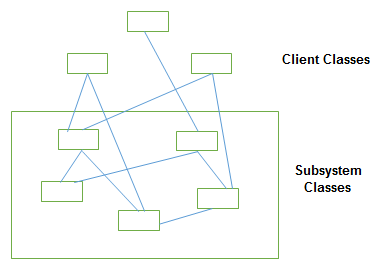
\includegraphics[scale=0.6]{./images/problem.jpg}
		\end{column}
	
		\begin{column}{.5\textwidth}
			\begin{itemize}
				\item You must make your code work with a broad set of objects that belong to a sophisticated library or framework.
				\item You’d need to initialize all of those objects, keep track of dependencies, execute methods in the correct order, and so on.
				\item As a result, the business logic of your classes would become tightly coupled to the implementation details of 3rd-party classes, making it hard to \textbf{comprehend and maintain}.
			\end{itemize}
		\end{column}
	\end{columns}
\end{frame}

\begin{frame}{Solution: Facade Pattern}
	\begin{columns}[T]
		\begin{column}{.5\textwidth}
			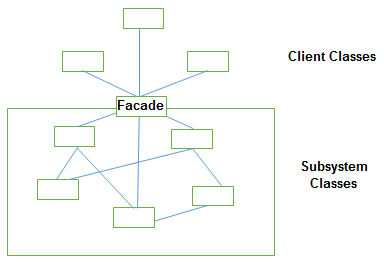
\includegraphics[scale=0.6]{./images/solution.jpg}
		\end{column}
	
		\begin{column}{.5\textwidth}
			\begin{itemize}
				\item A facade is a class that provides a simple interface to a complex subsystem.
				\item Provide limited functionality in comparison to working with the subsystem directly
				\item Having a facade is handy when you need to integrate your app with a sophisticated library that has dozens of features, but you just need a tiny bit of its functionality.
			\end{itemize}
		\end{column}
	\end{columns}
\end{frame}

\begin{frame}{The Intent of Facade Design Pattern}
	\begin{center}
	\textcolor{red}{\textbf{Provide a unified interface to a set of interfaces in a subsystem. Facade defines a higher-level interface that makes the subsystem easier to use.}}\\
	\end{center}
\end{frame}

\begin{frame}{Structure of Facade Pattern: Object adapter}
	\begin{center}
	\begin{tikzpicture}
 	\umlemptyclass[x=0,y=0]{Client}
 	\umlclass[x=3,y=0]{Facade}{}{operation()}
 	\umlclass[x=9,y=0]{AdditionalFacade}{}{addOperation()}
 	\umlclass[x=0,y=-5]{SubSystem1}{}{}
 	\umlclass[x=3,y=-5]{SubSystem2}{}{}
 	\umlclass[x=6,y=-5]{SubSystem3}{}{}
 	\umlclass[x=9,y=-5]{SubSystem4}{}{}
 	\umluniassoc[pos=0.95, align=right, name=uniassoc]{Client}{Facade}
 	\umluniassoc[pos=0.95, align=right, name=uniassoc]{Facade}{AdditionalFacade}
 	\umluniassoc[geometry=|-|, pos=0.95, align=right, name=uniassoc]{Facade}{SubSystem1}
 	\umluniassoc[geometry=|-|, pos=0.95, align=right, name=uniassoc]{Facade}{SubSystem2}
 	\umluniassoc[geometry=|-|, pos=0.95, align=right, name=uniassoc]{Facade}{SubSystem3}
 	\umluniassoc[geometry=|-|, pos=0.95, align=right, name=uniassoc]{AdditionalFacade}{SubSystem4}
	\end{tikzpicture}	
	\end{center}
\end{frame}

\begin{frame}{Sequence Diagram}
\begin{center}
	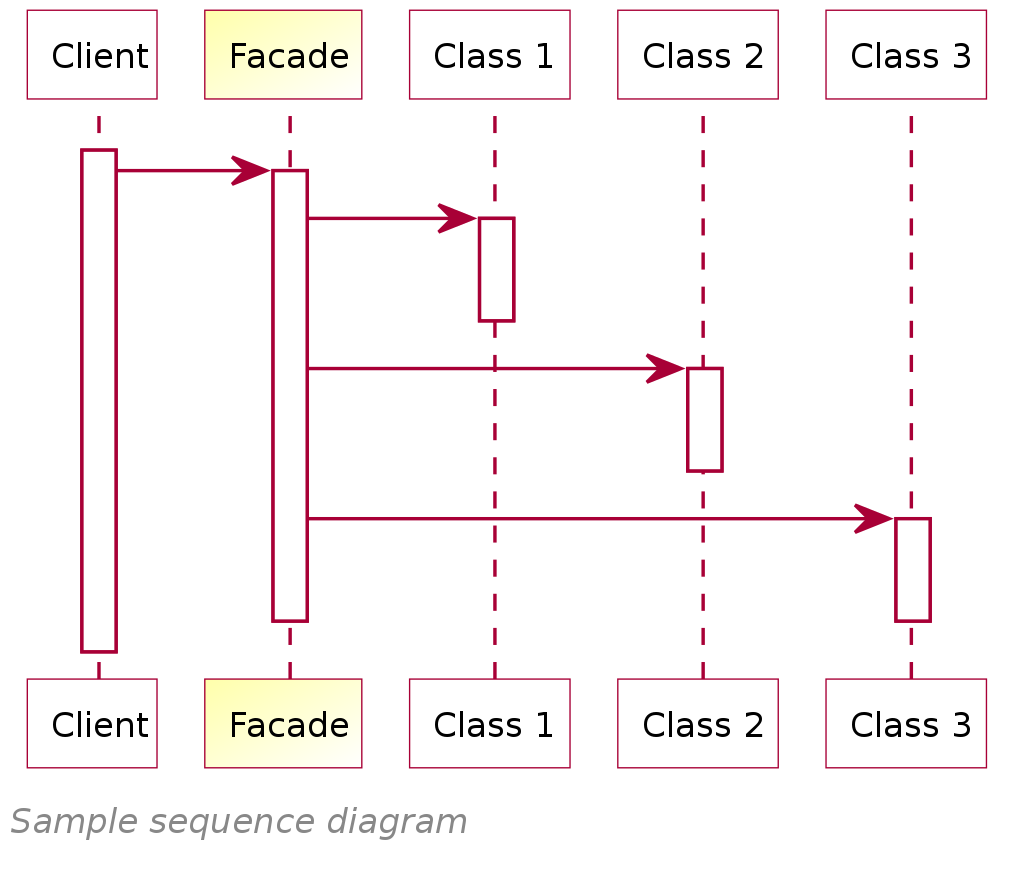
\includegraphics[scale=0.25]{./images/sequence.png}
\end{center}
\end{frame}

\begin{frame}{Basic implementation: cpu class}
\begin{columns}[T]
\begin{column}{.45\textwidth}
\lstset{basicstyle=\tiny,style=myCustomCppStyle}
cpu.h
\lstinputlisting{./examples/cpu.h}
\end{column}

\begin{column}{.45\textwidth}
\lstset{basicstyle=\tiny,style=myCustomCppStyle}
cpu.cpp
\lstinputlisting{./examples/cpu.cpp}
\end{column}
\end{columns}
\end{frame}

\begin{frame}{Basic implementation: memory class}
\begin{columns}[T]
\begin{column}{.45\textwidth}
\lstset{basicstyle=\tiny,style=myCustomCppStyle}
memory.h
\lstinputlisting{./examples/memory.h}
\end{column}

\begin{column}{.45\textwidth}
\lstset{basicstyle=\tiny,style=myCustomCppStyle}
memory.cpp
\lstinputlisting{./examples/memory.cpp}
\end{column}
\end{columns}
\end{frame}

\begin{frame}{Basic implementation: hard driver}
\begin{columns}[T]
\begin{column}{.45\textwidth}
\lstset{basicstyle=\tiny,style=myCustomCppStyle}
hardDriver.h
\lstinputlisting{./examples/hardDriver.h}
\end{column}

\begin{column}{.45\textwidth}
\lstset{basicstyle=\tiny,style=myCustomCppStyle}
hardDriver.cpp
\lstinputlisting{./examples/hardDriver.cpp}
\end{column}
\end{columns}
\end{frame}

\begin{frame}{Basic implementation: computer facade}
\begin{columns}[T]
\begin{column}{.45\textwidth}
\lstset{basicstyle=\tiny,style=myCustomCppStyle}
computerFacade.h
\lstinputlisting{./examples/computerFacade.h}
\end{column}

\begin{column}{.45\textwidth}
\lstset{basicstyle=\tiny,style=myCustomCppStyle}
computerFacade.cpp
\lstinputlisting{./examples/computerFacade.cpp}
\end{column}
\end{columns}
\end{frame}

\begin{frame}{Applicability}
	\begin{itemize}
		\setlength\itemsep{1em}
		\item  Use the Facade pattern when you need to have a limited but straightforward interface to a complex subsystem.
		%Often, subsystems get more complex over time. Even applying design patterns typically leads to creating more classes. A subsystem may become more flexible and easier to reuse in various contexts, but the amount of configuration and boilerplate code it demands from a client grows ever larger. The Facade attempts to fix this problem by providing a shortcut to the most-used features of the subsystem which fit most client requirements.
		\item Use the Facade when you want to structure a subsystem into layers.
		%Create facades to define entry points to each level of a subsystem. You can reduce coupling between multiple subsystems by requiring them to communicate only through facades.
	\end{itemize}
\end{frame}

\begin{frame}{How to Implement}
	\begin{itemize}
		\setlength\itemsep{1em}
		\item Check whether it’s possible to provide a simpler interface than what an existing subsystem already provides. 
		%You’re on the right track if this interface makes the client code independent from many of the subsystem’s classes.
		\item Declare and implement this interface in a new facade class. The facade should redirect the calls from the client code to appropriate objects of the subsystem. The facade should be responsible for initializing the subsystem and managing its further life cycle unless the client code already does this.
		\item To get the full benefit from the pattern, make all the client code communicate with the subsystem only via the facade. Now the client code is protected from any changes in the subsystem code.
		%For example, when a subsystem gets upgraded to a new version, you will only need to modify the code in the facade.
		\item If the facade becomes too big, consider extracting part of its behavior to a new, refined facade class.
	\end{itemize}
\end{frame}

\begin{frame}{Pros and Cons}
	\begin{columns}[T]
		\begin{column}{.5\textwidth}
			\begin{itemize}
				\item You can isolate your code from the complexity of a subsystem.
			\end{itemize}
		\end{column}
	
		\begin{column}{.5\textwidth}
			\begin{itemize}
				\item A facade can become a god object coupled to all classes of an app.
			\end{itemize}
		\end{column}
	\end{columns}
\end{frame}

\begin{frame}{Relations with Other Patterns}
	\begin{itemize}
		\setlength\itemsep{1em}
		\item Facade defines a new interface for existing objects, whereas Adapter tries to make the existing interface usable. Adapter usually wraps just one object, while Facade works with an entire subsystem of objects.
		\item Abstract Factory can serve as an alternative to Facade when you only want to hide the way the subsystem objects are created from the client code.
		\item Flyweight shows how to make lots of little objects, whereas Facade shows how to make a single object that represents an entire subsystem.
		\item Facade and Mediator have similar jobs: they try to organize collaboration between lots of tightly coupled classes.
		%Facade defines a simplified interface to a subsystem of objects, but it doesn’t introduce any new functionality. The subsystem itself is unaware of the facade. Objects within the subsystem can communicate directly.
		%Mediator centralizes communication between components of the system. The components only know about the mediator object and don’t communicate directly.
		\item A Facade class can often be transformed into a Singleton since a single facade object is sufficient in most cases.
		\item Facade is similar to Proxy in that both buffer a complex entity and initialize it on its own. Unlike Facade, Proxy has the same interface as its service object, which makes them interchangeable.
	\end{itemize}
\end{frame}

\begin{frame}
\begin{center}
{\fontsize{40}{50}\selectfont Thank You!}
\end{center}
\end{frame}

\end{document}
